%%%%%%%%%%%%%%%%%%%%%%%%%%%%%%%%%%%%%%%%%%%%%%%%%%%%%%%%%%%%%%%%%
%		Audio plugins architectures 			                %
%								                                %
%								                                %
%	Authors of this document: Remy Muller & Vincent Goudard     %
%					 			                                %
%%%%%%%%%%%%%%%%%%%%%%%%%%%%%%%%%%%%%%%%%%%%%%%%%%%%%%%%%%%%%%%%%

\documentclass[12pt,a4paper]{report}

\newif\ifpdf
\ifx\pdfoutput\undefined
\pdffalse % we are not running PDFLaTeX
\else
\pdfoutput=1 % we are running PDFLaTeX
\pdftrue
\fi

\ifpdf
\usepackage[pdftex]{graphicx}
\else
\usepackage{graphicx}
\fi

\usepackage{a4}
\usepackage{helvet}
\usepackage[latin1]{inputenc}
\usepackage{amsmath}
\usepackage{amsfonts}
\usepackage{array}
\usepackage{color}

%-----------------------------------------------------------
% customize header
%-----------------------------------------------------------
\usepackage{fancyhdr}
\pagestyle{fancy}
% with this we ensure that the chapter and section
% headings are in lowercase.
\renewcommand{\chaptermark}[1]{\markboth{#1}{}}
\renewcommand{\sectionmark}[1]{\markright{\thesection\ #1}}
\fancyhf{} % delete current setting for header and footer
\fancyhead[LE,RO]{\bfseries\thepage}
\fancyhead[LO]{\bfseries\rightmark}
\fancyhead[RE]{\bfseries\leftmark}
\renewcommand{\headrulewidth}{0.5pt}
\renewcommand{\footrulewidth}{0pt}
\addtolength{\headheight}{0.5pt} % make space for the rule
\fancypagestyle{plain}{%
\fancyhead{} % get rid of headers on plain pages
\renewcommand{\headrulewidth}{0pt} % and the line
}
%-----------------------------------------------------------%


\newtheorem{theorem}{Theorem}
\newtheorem{corollary}[theorem]{Corollary}
\newtheorem{definition}{Definition}

\title{\textbf{Real-time audio plugin architectures}\\
\large a comparative study\\
---\\
IRCAM -- Centre Pompidou \\}
\author{Vincent Goudard and Remy Muller}

% Create hypertext links for each chapter in the contents page
\usepackage[pdftex,bookmarks]{hyperref}

%------------------
\newcommand{\code}[1]{\texttt{#1}}

\begin{document}

\ifpdf
\DeclareGraphicsExtensions{.pdf, .jpg, .tif}
\else
\DeclareGraphicsExtensions{.eps, .jpg}
\fi

\maketitle

%--------------------------- Abstract -----------------------------
\cleardoublepage
\begin{abstract}
\noindent This document is born after a study of the existing standards for real-time audio plugins. It aims at giving an idea of the underlying structure behind all these incompatible standards, and pointing out differences when they occur.
\end{abstract}


%----------------------- Table of contents  -----------------------
\cleardoublepage

\tableofcontents

%***************************************************************************
% Introduction of pluginarch.tex
% Authors: Remy Muller & Vincent Goudard
%***************************************************************************

\chapter{Introduction}
\noindent Currently, there is more than ten audio \textit{plugin standards}, basically one per major host manuacturer such as Steinberg or Digidesign but Microsoft and Apple have also developped multimedia APIs\footnote{Application Programmers Interface.} integrated to their OS\footnote{Operating System.} that include audio plugins. These standards share a lot of features and behaviours while remaining incompatible. Many converters have been released these last years for breaking those incompatibilities, but they have some unwanted drawbacks: they increase the CPU charge and they are often limited to an OS. In addition, porting plugins from an OS to another does take time especially when dealing with graphics or filesystem access. Many people have tried for their own use to develop tools to abstract from the plateforms and the standards when developping plugins, thus reducing the cost of developpement and easing developers' life. Unfortunately few of these tentatives have been released publically.\\

\noindent The purpose of this document, beyond plugin formats, is to identify what is the specificity of audio plugins, what is common to all standards and what may differentiate them.\\

\noindent We do not pretend to write a tutorial for writing cross-plateform/cross-standards plugins nor to be exhautive but rather give an overview of what one may encounter when trying to target different plateforms and standards, and look for a common model that can be extracted.

%----------------------------------EOF-------------------------------------%
%***************************************************************************
% Chapter 2 of pluginarch.tex
% Authors: Remy Muller & Vincent Goudard
%***************************************************************************

\chapter{What is an audio plugin?}


%---------------------------------------------------------------------------
\subsubsection{What is its purpose?}
\noindent A plugin is intended to extend an audio creation environment by the use of dedicated third party libraries. Thus any user should be able to find plugins that fits perfectly their needs to customize this environment. Typically plugins can be considered as \textit{virtual devices} based on the analogy with hardware devices such as reverbs, compressors, delays, synthetizers, samplers or beatboxes that can be connected together in a modular way. This allows host manufacturers to focus on the conviviality and efficiency of their products while specialized manufacturers rather focus on the \textit{Digital Signal Processing} part.

\subsubsection{Approaches}
We can distinguish 3 approaches to do plugins
\begin{itemize}
\item Plugins integrated into a multimedia API like Apple's Audiounits and Microsoft's DirectX. 
\item Plugins related to a reference host like VST, RTAS, MAS\footnote{respectively cubase, protools and digital performer}. Some of them can be found on different plateforms like VST or RTAS.
\item Modules attached to modular softwares like the "Max family"\footnote{Cycling 74's Max/Msp, Ircam's jMax an CRCA's Pure Data.}, Buzz or EyesWeb.
\end{itemize}
We should also consider LADSPA on GNU-linux which is the de-facto standard for that plateform but that can not be attached to any  of the above categories.


%---------------------------------------------------------------------------
\section{General model}
\noindent A plugin treats an \textbf{audio signal} then it needs to be \textbf{controlled} and in order to work in a host environment, host and plugin have to know their repective {setup \& properties}.\\
The audio stream is usually treated by blocks (buffers) inside whom samples are synchronous to the samplerate. In general, control parameters have a lower refresh rate and can be either treated between audio blocks -- on-demand -- if the value has changed, or queued with time-stamps relative to a position in a block for audio-rate resolution. Properties are mostly static flags but some can be dynamic though.\\

\begin{figure}[htb]
\begin{center}
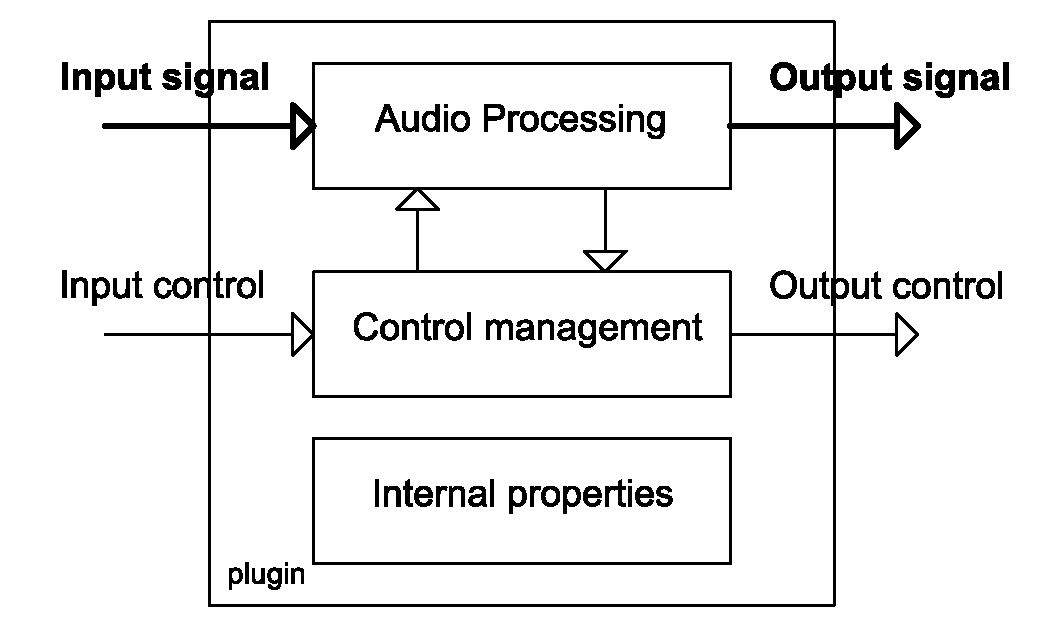
\includegraphics[height=2.5in,width=4.16in]{pluginmodel}
\caption{A common model behind musical plugin architetures}
\end{center}
\end{figure}

\subsubsection{Setup \& properties}
\noindent Plugins have to know about the host's capabilities like sending/receiving events, providing multichannels busses\ldots  In addition there are lot of situations where we would appreciate that plugins can know more about the \textit{musical context} (i.e. tempo, score-position, metric\ldots) than just audio and control data.\\
\noindent The plugin has to give information about its ins/outs, their specificities such as side-chain, mono, stereo or surround and many things such as its latency\footnote{An algorithm like a Fourrier Transform may introduce a pure delay in the signal chain because it needs a minimum number of sample to start. In a sequencer (not in real-time!) this pure delay can be compensed by the host by sending data to the plugin in advance.} or its tail-time\footnote{Basically all the algorithms based on convolution may introduce a tail i.e. output samples even when there is no more input data (e.g. a delay, a reverb a FIR filter\ldots)}. There is also some hosts that allow plugins to give them commands such as \textit{play, stop or set tempo} but it is not really wide-spread. 


%---------------------------------------------------------------------------
\section{Inputs -- Outputs}
 
\noindent To understand what is relevant to determine the number and the kind of IOs, we may analyse what plugins algorithms does around 3 different of kind functionnalities -- analysis (\textbf{A}), transformation (\textbf{T}) and synthesis (\textbf{S}) -- that can be either alone or mixed together in the same entity.\\

\begin{figure}[htb]
\begin{center}
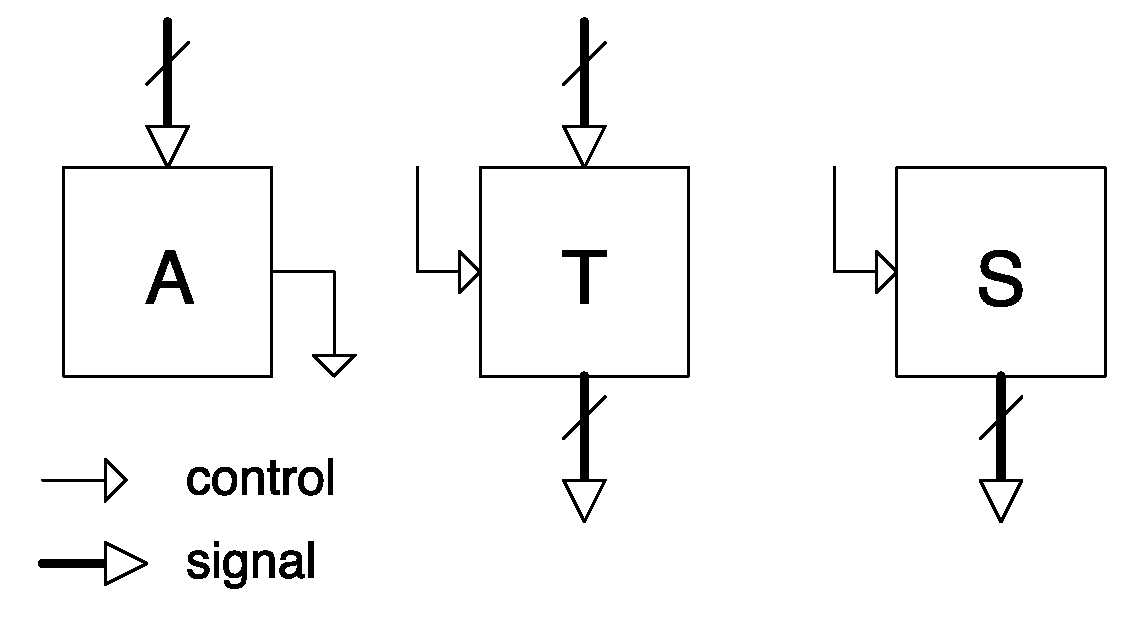
\includegraphics[height=1.2in,width=2.2in]{functions}
\caption{functions}
\end{center}
\end{figure}  

\noindent Moreover, plugin setups highly depend on what the host allows and how the plugin will be attached to its environment. While most hosts only support mono and stereo (even if surround begins to be popular with  the recent success of the DVD and the famous 5.1 surround format\footnote{left, center, right, rear left, rear right plus subwoofer}), we can also distinguish between effects that will be treated as \textbf{inserts} (integrated in a chain on a single bus), \textbf{sends} (they can be shared by many voices in a mixing-console and the output is summed on the master bus), \textbf{instruments} (no audio input) or simply integrated into a modular host.

\subsubsection{Audio}
\noindent The number of \textbf{audio inputs and outputs} vary from one plugin to another, they can be grouped into busses that can be mono, stereo, surround\ldots but they mostly depends on the host capabilities. Moreover, in some standards -- the number is still growing --, it is possible to define side-chain\footnote{a side-chain channel can be analyzed or used directly to modify the main audio stream processing.} (see figure \ref{sidechain}). 

\begin{figure}[htb]
\begin{center}
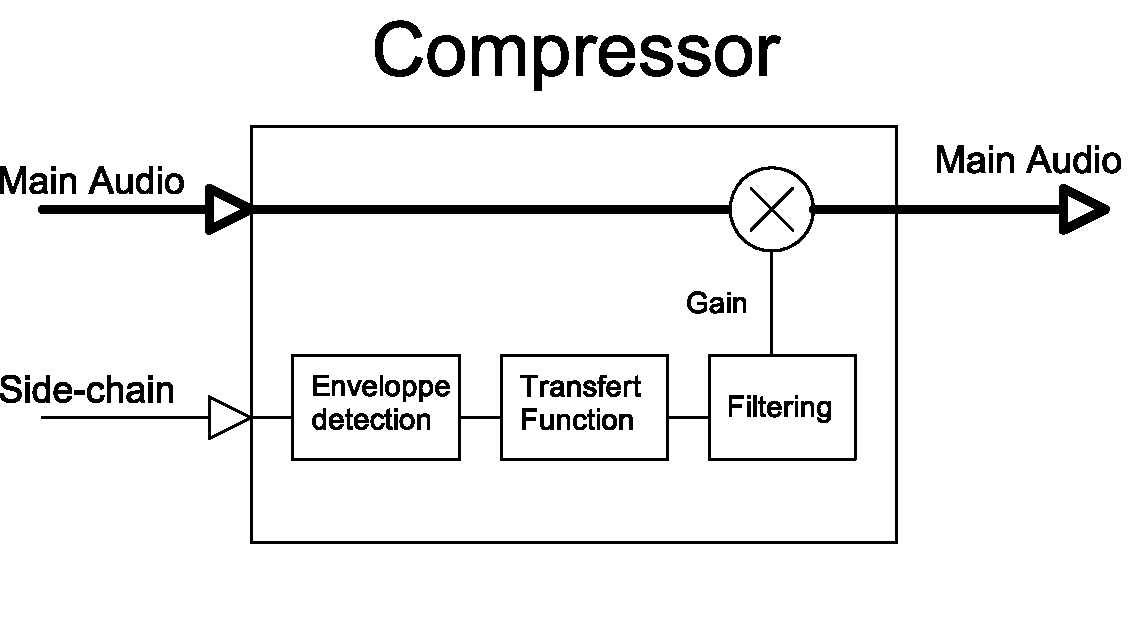
\includegraphics[height=2in,width=3.5in]{sidechain}
\caption{A side-chain example: a compressor}
\label{sidechain}
\end{center}
\end{figure}  

\subsubsection{Control}
\noindent Though it is possible to build a plugin that has no way to be controlled, like a phase inverter, it is of limited interest in a musical context where tweaking the parameters or sending notes is part of the creation. You may want to both change the plugin's parameters and record their variation for later playback. Hence most plugins should provide control input and output at the same time. Most of the time hosts and plugins notify each other of parameters' evolution in a simple way but one can also find callback and polling mechanisms. In addition sending \textbf{control data} between plugins can sometimes be performed either directly via parameters (LADSPA) or by an event-oriented protocol like MIDI (VST).\\

%---------------------------------------------------------------------------
\section{The ``process"}
\noindent All plugins have this function in common often called ``process''. This is where the most important thing happens: \textit{audio processing}.
All the current standards treat audio as input and output buffers (of given length), that can be given as floating-point sample arrays, or by more sophisticated structures with additionnal information. Processing can be in-place, in which case in and output buffers are the same (i.e. they share the same memory location, processing is thus destructive.), or buffer-to-buffer, where they are different in this case it is possible to have either accumation (send effects) or replacing (inserts). Parameters are usualy known before the process starts, but you may have to update them by hand. For simple audio processing like biquadratic filtering, it should be enough to use directly the buffer provided, but when doing FFT processing for example you may want to re-buffer audio samples to fit your internal buffer size in which case you may introduce additionnal latency in the signal chain.

%...........................................................................
\section{The user interface}
\noindent The GUI should be considered at least as important as the audio processing algorithm because it is the filter thru wich your plugin will be perceived. It is a key-point for the conviviality and usability of a plugin, everything should be fast and easily tuneable in a precise way with a convenient visual feedback. In particular, parameters' mapping can really make the difference in the way people feel about how your plugin sounds.\\
% citer les �tudes psycho-acoutiques sur l'influence du mapping.
The GUI can be either generated automatically by the host with the help of the information or hints that the plugin can provide about itself (its  parameters type, their range and units\ldots, and the type of control that should be used -- slider, combo-box, switch, knob, 2D controler, \ldots --) or provided by the plugin manufacturer to reach a higher level of customization.\\
However we will skip the GUI topic in this document. We consider control parameters as the plugin interface without taking account the way these parameters are changed by the user.

%...........................................................................
\section{Plugin developpement}
\noindent The API defines the layer through which plugins and hosts can see each other and also the tools that can be used to ease the developpement step.\\
The Host needs different information than the user about plugins such as their ID, their capabilities, their setup, the number of parameters or their names. The host needs to receive computer-readable data in the way it is programmed to. In addition most of the SDKs\footnote{Software Developpement Kits.} provide a set of tools, functions, utilities. In the same effort, they often allow the use of OOP\footnote{Object Oriented Programming.} languages such as C++, ObjectiveC or Pascal to ease the modelisation step and the tasks distribution inside a same plugin.
%----------------------------------EOF-------------------------------------%
%***************************************************************************
% Chapter 3 of pluginarch.tex
% Authors: Remy Muller & Vincent Goudard
%***************************************************************************

\chapter{The signal stream}



%---------------------------------------------------------------------------
\section{Nature of the signal stream}

%...........................................................................
%\subsection{Type - range}
\noindent Most of the time, the signal stream is represented as floating-point samples in the intervall $[-1;1]$ full-scale. However some standards supports fixed-point samples\footnote{e.g. The CD format uses 16-bit signed integer samples allowing signal to be coded in the intervall $[2^{15}-1;-2^{15}]$ while the DVD uses 24-bit ones: range=$[2^{23}-1;-2^{23}]$} for historical or technical\footnote{DirectX, AudioUnits and TDM supports fixed-point samples because their plugins may deal directly with files, cd-rom, dvd-rom, soundcards or fixed-point DSP while other standards only deals with hosts for whom the floating point representation is more convenient.} reasons .\\
For efficiency purpose, those samples are packed into buffers whose size can be fixed or variable from one call to the other. Though sample-by-sample processing\footnote{It allows feedback and recursion between objects and is very useful for `physical modeling'} is already used in some DSP libraries, there isn't already any standard doing the processing that way. The samplerate is supposed to be constant (and known) at least during the length of the buffer and may change at the buffer-rate though it is unusual\footnote{typically values like 44,1kHz for the CD, 48kHz for DAT or video and 96kHz for the DVD are used.}.\\
Audio buffers can either be surrounded by additionnal information like time-stamps\footnote{It can be used for synchronisation purpose by the host scheduler when many complex audio paths are present.}(DXi, EyesWeb, AU), samplerate, buffer-size\ldots  or transmitted (most of the time) as simple arrays.\\ % TODO: who implements : sr, buffersize ...etc
Some plugin API -- DX, AU -- allow channels interleaving for compatiblity with files types and streaming protocol, but it is quite marginal and tends to disappear at least for real-time processing. The most common (and easiest) way is to transmit channels as separated mono buffers.



%---------------------------------------------------------------------------
\section{Signal processing}

\noindent Here we come to most important part of a plugin, almost every plugin standards have the same method called \verb|process()| to do the audio processing, only the way it is called and the arguments are different between standards. This method is either called directly by the host or by the next plugin in the chain in the case of graph-oriented hosts. Input and output buffers are, most of the time, provided by the host and can either be the same or different to allow in-place or buffer-to-buffer processing but the plugin can't assume one or another and should work correctly in both cases or specify if it suports it (LADSPA).\\

\noindent As a major difference with hardware Digital Signal Processors, this method is assumed to be non interruptible. Therefore parameters interpolation (if needed) or other sample-accurate processing has to be done inside the process and can't be done automatically since processing audio by buffers prevent from audio-rate control as soon as the buffer-size exceeds 1 sample.



%...........................................................................
\section{General considerations about Digital Signal Processing}
\noindent This section doesn't plan to explain rules of `audio processing algorithm optimization'. We just want to explicitely note that since audio-rates are measured in tenth of kHz and that plugins may handle several channels, the number of samples to process can become huge, thus one should pay special attention to the DSP algorithm complexity\footnote{In particular algorithms whose complexity is exponential or polynomial with the number of sample to process, shouldn't be used in a real-time context.}.\\

\noindent Without going into assembler coding, one should avoid memory allocations, conditional expressions inside loops\footnote{It can break pipe-lining optimizations}, too many non-static-inline-function calls or intensive float--int conversion among other general programming tips. Note that in a lot of case down-sampling during the analysis step (e.g. in envelope detection) can save precious CPU time for other purpose.

%----------------------------------EOF-------------------------------------%

%***************************************************************************
% Chapter 4 of pluginarch.tex
% Authors: Remy Muller & Vincent Goudard
%***************************************************************************

\chapter{Control}

\noindent The control interface allow the user to act on parameters, to tune the behaviour of the audio processing function. This can be done in real-time, so that the user can directly hear the consequence of his changes on the audio signal transform.\\
\noindent There are different kinds of parameter, that require different handling. We can consider three main categories of parameters:
\begin{itemize}
\item{\textbf{Continuous parameters:}} These parameters can be characterized by the fact that they do not introduce a discontinuity in the audio stream \footnote{A dicontinuity in the audio stream is characterized by audible `zipper noise' or `clicks'}, when they change of a small amount. As a consequence, these parameters can be interpolated. These parameters are obviously represented by numerical values and can be considered `passive', in the sense that they are just used as a variable value in a generic computation. As examples: a filter's cutoff-frequency, a volume gain, a modulation frequency or a clipping threshold are continuous.

\item{\textbf{Events:}} These parameters, sometime referred to as \textbf{messages} or \textbf{commands}(EyesWeb), are characterized by their discrete nature. These messages can be of any type, but should belong to a set of predefined messages, known from the plugin. They are not directly used in computation, but are rather interpreted to trigger a specific action, without breaking the audio stream process. As examples: the choice between `sawtooth', `sine', and `square' for a modulator signal, a MIDI note-on event or the number of echoes in a delay.

\item{\textbf{Setup parameters:}} These parameters affects the plugin's configuration. They are non-realtime because they involve computationally expensive operations, like memory allocation, that definitely break the audio signal stream. As exemples: the choice of a impulse response file for a convolution plugin or a fft-size in a frequency domain transform.
\end{itemize}

\noindent This distinction between these three categories is not always that clear and well defined, but these three kinds of parameter correspond to different handlings.\\

\noindent With the increase of complexity of the plugins, which require more and more internal parameters to get finer acoustic results\footnote{e.g. in physical-modelling of instruments, reverb rooms...}, there is an ongoing need of mapping and conversion routines, so that the user can still control them in an ergonomic manner. The parameters available to the user and the host (\textbf{external parameters}) can differ from the parameters used in the process computation (\textbf{internal parameters}). There may exist a conversion layer between them.This conversion can be of various kind, such as scaling a gain expressed in dB to a linear scale, mapping of frequency, gain and resonance to filter coefficients or clipping of the parameter to its range.\\


%---------------------------------------------------------------------------
\section{External parameter declaration}
%...........................................................................
\subsection{Mandatory declarations}
\noindent The external parameters should be declared, to allow the host and/or the user to modify them. However, the host and the user do not need the same information to handle them.
The minimum required set of parameters properties that the host should know contains, at least, the two following:
\begin{itemize}
\item{\textbf{The parameter ID}}: This ID is used as a selector among the parameter structure. Parameters ID are signed or unsigned long integers in all major audio plugin standards, sometimes of an enumerated type (DXi, VST, RTAS).

\item{\textbf{The type}}: LADSPA and VST make use of 32-bit float only for all control data, and VST restrict the range to [0,1]. Other standards like DXi and AudioUnits implement all parameters as 32-bit float for efficiency, but keep a field in a parameter info structure, that defines whether to interpret the value as an integer, floating-point value, boolean, or enumeration (integer series). We find a similar mechanism in EyesWeb, but with three base format: double, int, and character string, plus a `Parameter type' flag.\\
% MAS : long, short, char, byte, bool, floatIEEE and float as text.
% RTAS ??
% !!!!! check that is is not fake like DX, and AU!!!!!
\end{itemize}


%...........................................................................
\subsection{Optional declarations}
\noindent Most plugin standards do offer much more information about parameters, to prevent the host and the user from manipulating them wrongly, and to let the user access them in a friendlier way. Such information may be stored in a `ParameterInfo' structure (DXi, AU), or suggested as defined flags or `hints' (LADSPA).

\begin{itemize}
\item{\textbf{The name or label}} is interesting for the user who do not speak like machines\ldots The parameter name can be part of a parameter information structure, like in DXi, EyesWeb and AU. LADSPA stores the port names (audio AND control) in an array. Parameter's name is not mandatory in VST, but a `GetParameterName' method exists in the API, that the developper can implement.
% MAS: ???

\item{\textbf{The units}} gives more sense to the values. Few standards offer this feature: DXi,and EyesWeb stores the unit of each parameter in the ParamInfo structure. In AU, the units is part of the type: for example the type `angle' is expressed in degrees or radians, the type `frequency' in Hertz\ldots and the parameter's mapping is chosen with respect to this.
% MAS : ????

\item{\textbf{The range}}: It gives hints about what values this parameter is assumed to take. This is useful to prevent the plugin from doing error-leading computations, like log(0), negative frequency for a filter \ldots etc. It also helps the user to grasp the meaning of the parameter he's handling. Almost all standards allow to specify the range of the parameters, except VST for which the range is normalized between [0;1] and conversion has to be done by hand. 

\item{\textbf{A default value}}: It can initialize the parameter to a relevant value, within the parameter range, at instantiation time. This feature is implemented in LADSPA, DXi, EyesWeb AU, MAS. In VST, it is stored in the default preset.
% RTAS :  ???

\item{\textbf{The mapping}}: It helps manipulating the parameter in a more ergonomic way. For example, frequency and gain are often more convenient when handled with logarithmic mapping. Mapping may be linear (all standards), logarithmic (LADSPA, AU), boolean (LADSPA, DXi, AU), indexed (LADSPA, DXi, AU)\ldots VST provides conversion tools for GUI-display only.
% EYESWEB : no mapping in the API

\item{\textbf{Automation\footnote{See \ref{automation} for explanation.}}}: Automatable parameters have to be declared as such by the apropriate mean:
\begin{itemize}
\item{AudioUnits}: Flag in the parameter information structure.
\item{DXi}: Index of automated parameters should be less than\\
\verb|NUM_AUTOMATED_PARAMS| within the parameters enumeration.
\item{MAS}: Automated parameters should be public.
\item{VST}: During run-time, one should use the specific method\\
\verb|setParameterAutomated|.
\end{itemize}
% RTAS : ??
\end{itemize}


\begin{table}
{\scriptsize
\begin{tabular}{|l|c|c|c|c|c|}
\hline
          & Name/Label        &  Units         & Range               & Default        & Mapping          \\
\hline
VST       &Not mandatory, but &  ---           & [0,1] fixed         & ---            & conversion tools \\
          & method in the API &                &                     &                & for display only \\
\hline
AU        & In a ParamInfo    & In a ParamInfo & Min, max stored in  & In a ParamInfo & Many many!       \\
          & structure         & structure      & ParamInfo struct    & structure      &                  \\
\hline
LADSPA    & In the PortNames  &  ---           & min and  max        & suggested as   & lin,log,int,     \\
          & array             &                & suggested as hints  & hint, relative & bool,SR-multiple \\
\hline
MAS       & ???               & ???            &  ???                & ???            & No               \\
\hline
DXi       & In a ParamInfo    & In a ParamInfo & Min, max stored in  & In a ParamInfo & ---              \\
          & structure         & structure      & ParamInfo struct    & structure      &                  \\
\hline
EyesWeb   & In a ParamInfo    & In a ParamInfo & Flags HAS\_MIN\/MAX & Yes            & ---              \\
          & structure         & structure      & and values          &                &                  \\
\hline
RTAS      & ???               & ???            &  ???                & ???            & ???              \\
\hline
\end{tabular}
}
\caption{Available parameter information}
\end{table}

\noindent Many other meta-information can be found in some standards:\\
\textbf{EyesWeb} specifies with the help of flags, whether the parameter can be changed at design-time, at runtime (and if so, if it can be exported), and if it is initially disabled.\\
\textbf{AudioUnits} provides a really rich API, with many predefined types of parameters, which have their own units, mapping, and range. This include indexed, boolean, percent, second, phase, cent, decibel, hertz, pan, a general type which is float between 0.0 and 1.0, and others. The developper can also add his own types.


%---------------------------------------------------------------------------
\section{Parameter update}
\noindent The parameter update mechanism should efficiently take in account the fact that the parameter update rate\footnote{There is no `rate' in the strict sense, but we used this word for convenience.} is asynchronous in nature, in general significantly lower than the audio stream, and that many changes could occur at the same time. Some parameters are known in advance (e.g. like MIDI events in a sequencer track), and some are not (e.g. live actualisation through hardware knobs). \\
The parameter update can be represented as a two steps operation: external parameters which have changed must be sent to the plugin; then, a conversion -- if necessary -- must make the corresponding internal parameters available to the process in a correct format. The figure \ref{parameters} illustrates this mechanism.

\begin{figure}[htb]
\begin{center}
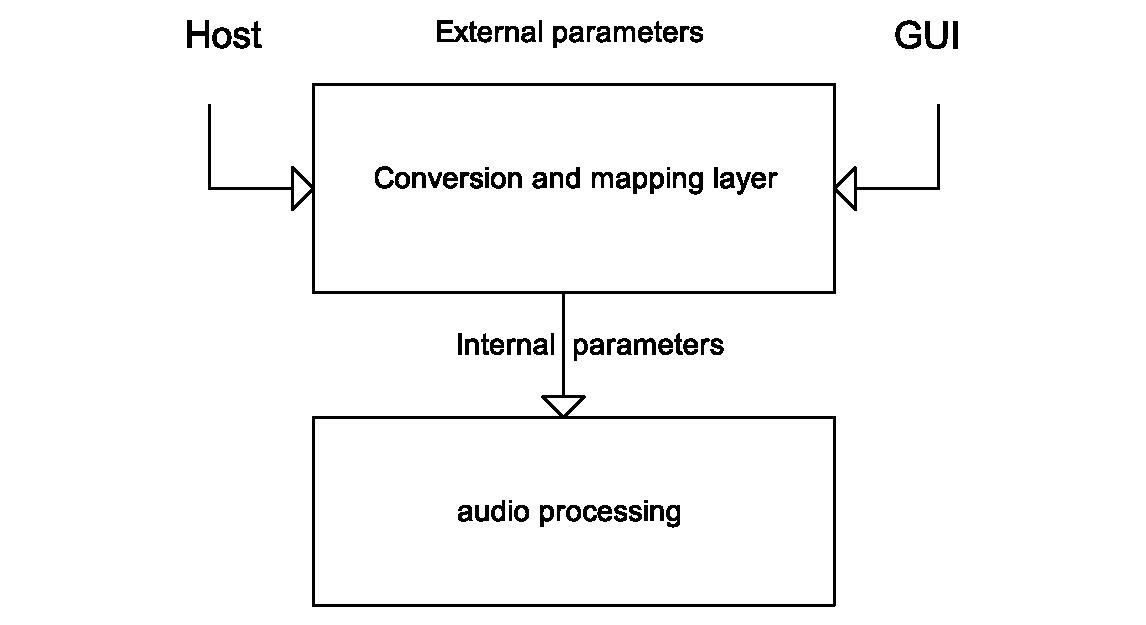
\includegraphics[height=3in,width=5in]{parameters}
\caption{Internal and external parameters}\label{parameters}
\end{center}
\end{figure}  

%...........................................................................
\subsection{Update mechanism}
% rate, sync/async, queues, timestamps ...

\noindent The most simple way to update parameters is the one implemented in LADSPA, and consists in a \textbf{polling mechanism}. At connection time, the host gives the plugin the adresses where it will write the external parameter values. The plugin can retrieve these values during the process function -- and only then --, assuming they may have changed. Everything that should be performed for mapping and conversion of these external parameters can only be done then.\\

\noindent In the second approach (VST, jMax), the host or the GUI calls a specific plugin method, usually called \verb|setParameter|. This method can only be called between two buffer processings. Necessary conversions and mappings should be implemented there by the plugin developer, so that internal parameters are up-to-date when the process function is called for the next buffer processing.\\

\noindent As a third case, some standards (DXi, AU) provide a conversion layer in the API between the plugin and the host or the GUI. Conversion and mapping are automatically done with the help of the parameter information structure. However, it is still necessary to retrieve the value of the parameters in the process function, and additionnal conversion have to be done here (e.g. computing filter coefficients from the cutoff frequency and the resonance, or checking mutual consistency of parameters).\\

\noindent Ways of handling events differ among plugin standards. A common and simple solution is to treat this set of value just like other parameters: reading and writing the value of the message with the \verb|GetParameter| and \verb|SetParameter| methods, and deciding on what should be done with a `\verb|case|' or `\verb|if|' condition. It can also be directly treated in the \verb|SetParameter| method (EyesWeb).



%...........................................................................
\subsection{Automation}
\label{automation}
\noindent The automation allow the user to record changes of parameters along a sequenced timeline, and play them back. These changes can be either recorded inline (i.e. in realtime, during playback) or offline (e.g. by editing graphically a curve on a sequenced track). The automation recording consists in taking the parameter's value every timeslice.\\
\noindent Most standards tends to allow this (DXi, AU, MAS, RTAS, VST) since it is a quite powerful tool. The parameters declared as automated parameters should be `realtime-able', i.e. they should not introduce too heavy computations or memory allocation. 

%...........................................................................
\subsection{Parameters encapsulation and meta data}

\noindent Some header-information might be provided to the plugin during runtime, in addition to the new parameter's value. Precisely, the time at which change occur, and the way the value should be modified can be specified.

\subsubsection{Type of data}
\noindent As it has been mentionned in the `Parameter declaration' section, some standard make use of a unique -or a restrained set of- data type for transport. In this case, a flag attached to the parameter in a parameter-info structure, specifies the type, into which the value should be casted.

\subsubsection{Timestamps}
\noindent The user who controls the interface can act at any time, disregarding what the plugin is doing. Thus, more than one change can occur during the time interval a timeslice is being processed. When considering punctual events such as audio attacks, synchronicity can play a major role in the audio rendition, and need more precision than the timeslice, which can last more than 50 ms.\\
\noindent Hence, timestamps can be attached to the parameter changes, to specify the precise sample accurate time at which they should occur. These events can be queued, their timestamp converted to the sample position within a buffer timeslice, and then be performed with the right time distribution during the next buffer processing.\\
\noindent In general, timestamping of parameters is limited to midi messages. Only EyesWeb make use of it for other control parameters.

\subsubsection{Interpolation}
\noindent On the other hand, for most parameters considered previously as `continuous', such a precision does not matter, since the audio timeslices are really small, but the continuous nature of the parameters should be respected to avoid `zipper noise' in the audio output signal. Therefore, various standards have implemented a way of interpolating the parameter' values to smooth the change, and avoid gaps in the audio stream that would generates these `clicks'. A common way of doing is to take in account the last value of the given parameter, and perform an interpolation between the new value and the previous one. Different kind of interpolation may be available to perform the interpolation such as linear (DXi, EyesWeb, AU) , quadratic (DXi) or sine (Dxi).\\
% TODO: which standard provide which interpolation?

% ---> What is given to the process function??   (derivative?, parameter buffer?)
% The DXi API  make use of the first and second derivative to interpolate the parameter's value between the bounds of the audio-buffer. Hence, the parameter's enveloppe is timestamped(?)\\
% EyesWeb modules provide a "Parameter smoothing" option.



%---------------------------------------------------------------------------
\section{Parameter persistence and presets}
\noindent Persistence of parameters is a saving of the parameters values, that enable the user to find these same values -- and not the default ones -- when the user re-open the plugin. It means that when the user close the host and relaunch it for a new session, the persistent parameters adjustments will be the same as when he quitted. This feature is useful when manipulating plugins with lots of control values, like an equalizer for example.\\
Presets are actually an extension of the persistence system to the user's will: the user can decide to store different sets of parameters that he likes, usually identifying them by a name. The way to store the preset depends on the presets size: if the preset is small, it can be stored by the host (VST) or in a register (DXi); whereas if the preset is bigger (e.g. it contains a waveform, or a picture), it will be stored in a separate file as a bytestream \footnote{The path of this file will be saved the same way a small preset would have been saved.}.\\


%---------------------------------------------------------------------------
\section{MIDI}
\noindent MIDI (Musical Instrument Digital Interface) is a protocol that transmits information about how music is produced. It is asynchronous but quantized at a maximum rate of 31,25 kbit/s\footnote{This rate was the standard for communication with hardware devices. However, hosts generally overcome this limitation internally: an adaptative resolution of 480 `ticks' per quarter-note is usual.}, and encode control values that fit in both \textit{event} (e.g. `note on/off') and \textit{continuous parameters} (e.g. `pitch bend') categories. As a major difference with GUI interaction, MIDI messages usually use time-stamps, allowing sample accurate rendering. One can distinguish different families among musical plugins using MIDI: synthesizers, MIDI-controlled effects, pure MIDI effects\footnote{MIDI effects consist in taking MIDI messages as data input and process them. No audio data is implied in the process. Most common MIDI effects are arpegiators, delays and echoes\ldots} and analysis plugins -- though those last ones aren't formalized in any standard for now -- depending on the kind of input and output data. In this document, we will only deal with synthesizers and MIDI-controlled effects.\\

%...........................................................................
\subsection{Synthesizers}
\noindent Synthesizers (or `instruments') appeared in the second generation of plugin standards. As harware ones, they get MIDI messages as input, usually have no audio input, and output audio data on many pins compared to chained effects. They often have a lot more parameters, and many of these ones are mapped to MIDI continuous controllers for a convenient live interaction.

%...........................................................................
\subsection{MIDI-controlled effects}
\noindent Integration of synthetizers into standards has allowed the interaction with plugins via MIDI. It allows to `play' an effect as an intrument, using the incoming audio as a primary material to generate sound. They are often intented for musicians more than sound-engineers. As examples we can cite filters whose cut-off frequency is tuned to MIDI notes, or live-samplers using the incoming audio as a wave-table.
%----------------------------------EOF-------------------------------------%

%***************************************************************************
% XSPIF user's guide -  userguide.tex
% Chapter : Standards specific considerations
% Authors: Remy Muller & Vincent Goudard
%***************************************************************************

\chapter{Standards specific considerations}

\section{VST}
\noindent With VST 2.3, the only way to output control, is to use MIDI
Continuous Controlers. For that purpose the values have to be
normalized in the range $[0-127]$, and then sent to the host as MIDI
data as defined by by the MMA\footnote{Midi Manufacturer Association
  \url{http://www.midi.org/}}. 

\section{Audio Units}
\noindent Control output is not yet featured in this standard, but
should come soon with Mac OSX 10.3 also called panther. 
Note that AudioUnit provides a set of predefined types -- namely
decibels, hertz, boolean, percent, seconds, phase, cents,
Degrees\ldots-- with the mapping done automatically. However, as XSPIF
can use arbitrary units with an arbitrary mapping, we only implemented
AudioUnit's ``generic parameters'' which only have a range and default
value with a linear mapping. Hence, if you specify a \emph{log}
mapping for a parameter, it will be ignored. Futur improvement to
XSPIF, could use the \emph{unit} -- which can be arbitraty -- attribute to guess the nature of the parameter.


\section{LADSPA}
\noindent In LADSPA, the control outputs undergo the same mechanism as
writing output audio buffers, and it consists in writing a float value
to a memory location which is or can be shared.\\ 
\noindent Thus, unlike VST and PD,  synchronicity is not ensured and
depends on the host management of the different threads. 

\section{PureData, Max/Msp, jMax}
\noindent With Pure data, Max/Msp and jMax, if the parameter's optionnal attribute
\verb|noinlet| is set to \emph{true}, it means that this specific
parameter will not appear as an inlet on the object's layout. It can
be useful if there are many parameters and you want to save space on
the screen to keep some visibility. However, this parameter will still
be controlable by sending the following message to the left-most inlet
\textit{parameter\_name} value. Note that, in pure data, the object
can also receive the message ``print'' which will display some
information about the plugin, in particular, the parameters' names,
and their range and the messages ``on'' and ``off'' which will call
respectively \emph{activate} and \emph{deactivate}.  
%*************************************************************************
% Conclusion of pluginarch.tex
% Authors: Remy Muller & Vincent Goudard
%*************************************************************************


\chapter{Conclusion}
\noindent As we have seen through this document, from an abstract point of view, plugins standards looks very similar and share a lot of functionnalities. Some are very quick and simple to develop, like LADSPA, leaving the hard work to the host and the user (GUI, mapping), while other like DirectX or RTAS, have a harder learning curve because they give (too?) many possibilities to the plugin manufacturers (Custom GUI, handling of control surfaces or onboard DSP, automation, MIDI\ldots). Between we can find AudioUnits and VST trying to make ends meet through easy APIs to start with, but allowing still many possibilities for (quite) experienced programmers.

\noindent However when looking into details, we can raise many differences. These differences are mostly dependent on the context in which the plugin standards were born. For historical, technical and commercial reasons, host manufacturers started on specific plateforms, targeting different kind of users and/or activities among audio-engineers, musicians, professionals, amateurs, post-production, multimedia, video \ldots. These initial constraints still remains present in standards because of backward-compatibility, despite the fact that since those early times companies and host have evolved, changed of plateform or even of customer's target.

\noindent In this specific context, the GMPI\footnote{Generalized Musical Plugin Interface} group was formed, at the end of 2002, on the initiative of Ron Kupper from Cakewalk and under the authority of the MMA\footnote{MIDI Manufacturer Association}, to design a new open and cross-plateform plugin standard, that would meet everyone needs, and put in common all the experience accumulated by people since the first host and plugin systems. However there is still a long way before we can use and develop for a unique kind of plugin that would be easy and quick to develop, highly scalable and efficient. In the meantime, developping for different standards and plateforms is still necessary and time-consuming. Furthermore the choice of the supported standards is fundamental to determine the audience that will be targeted.

%***************************************************************************
% Ressources for pluginarch.tex
% Authors: Remy Muller & Vincent Goudard
%***************************************************************************

\appendix

\chapter{Ressources}


\noindent Most of the ressources we used to write this study are available on the Internet. Here are the links to the web sites and SDK's of the principal standards:\\

\begin{itemize}
\item AudioUnits Site: \url{http://developer.apple.com/audio/} 
\item DirectX -- DXi Site: \url{http://www.thedirectxfiles.com/} 
\item EyesWeb Site: \url{http://infomus.dist.unige.it/eywindex.html} 
\item LADSPA Site: \url{http://www.ladspa.org/} 
\item jMax Site: \url{http://www.ircam.fr/jmax/} 
\item MAS Site: \url{http://www.motu.com/} 
\item Max/MSP Site: \url{http://www.cycling74.com/} 
\item PureData Site: \url{http://www.pure-data.org/} 
\item RTAS Site: \url{http://www.digidesign.com/} 
\item VST Site: \url{http://ygrabit.steinberg.de/} 
\end{itemize}


%--------------------------- bibliography  -------------------------
%\cleardoublepage
%\bibliographystyle{alpha}
%\addcontentsline{toc}{chapter}{\protect\numberline{}{Bibliography}}
%\bibliography{../xspif}

\end{document}
\end















